% ===========================================================================
%  gompertz_inhomogeneous.tex --- excised from the pathogenesis chapter.
%
%  SUGGESTED INSERTION POINT
%      CH2/sections/02_markov_chains.tex, inside \S m:sec:inhomogeneous:
%      after \S m:sec:logisticspeciation and before \S m:sec:coupled,
%      as a third worked example alongside the seasonal Lotka--Volterra
%      process and logistic speciation.
%
%  RATIONALE
%      Chapter 2 already owns the general result.  The trajectory below is
%      exactly the special case lambda(t) = beta*exp(-alpha*t) + gamma,
%      mu constant, of \cref{m:eq:meanodeinhom}; and the first-jump
%      computation is the same construction \S m:sec:logisticspeciation runs
%      for a different decaying rate.  It does no work in the pathogenesis
%      chapter, where it was the apparatus for a hypothesis
%      ("subductive proliferation") that chapter names and does not pursue.
%
%  NOTHING IN CHAPTER 2 HAS BEEN EDITED.  This file is an offer, not a
%  change; see PHASE_A_REPORT.md item 8.
%
%  Provenance: CH8/document MAIN/sections/01_opening.tex:166-278, including
%  the pgfplots figure at :202-230.
%
%  Corrections applied relative to the source:
%    * the missing minus sign in the ODE for p_0, three times (01:177, :178,
%      :190).  The stated solutions were already correct; only the displayed
%      equations were wrong.
%    * the rate is lambda(t) = beta*exp(-alpha*t) throughout; the source
%      introduced it as exp(-t) at :181, as exp(-alpha t) at :190, and gave
%      the answer with alpha = 1 implied at :192.
%    * the pgfplots ylabel at :209 closed its bracket one term early, so the
%      figure contradicted its own caption.
%    * the peak time is added; it was noted as an "interesting case" at :278
%      and not computed.
%    * notation is Chapter 2's: \ex, \pr, \ddt without \displaystyle, and no
%      bold scalars.
%    * the paragraph of thinking-aloud at :188 is cut to two sentences.
%
%  Labels use the m: namespace of Chapter 2, so that the file drops in.
% ===========================================================================

\subsubsection{Gompertz activation}
\label{m:sec:gompertz}

A third instance of the same construction is worth recording, because it
arises directly in the modelling chapters and because both of its principal
quantities are elementary. Let the rate of a time-inhomogeneous Poisson
process decay towards a floor,
\begin{equation}
\lambda(t)=\beta\ee^{-\alpha t}+\gamma,
\qquad
\alpha,\beta>0,\;\gamma\ge0,
\label{m:eq:gompertzrate}
\end{equation}
so that activation is initially rapid and settles to a baseline. The
decaying term represents reduced proliferation in response to recognition,
or to the using up of a resource; $\gamma$ is the baseline that remains.

\paragraph{The first jump.}
Write $p_i(t)=\pr{X_t=i}$. For the homogeneous Poisson process the state-zero
probability satisfies $p_0(t+\Delta t)=p_0(t)[1-\lambda\Delta t+o(\Delta t)]$
--- the probability of still being at zero at $t+\Delta t$ is the
probability of being at zero at $t$ and of nothing happening in
$(t,t+\Delta t]$ --- and in the limit
\begin{equation}
\ddt{p_0(t)}=-\lambda p_0(t),
\qquad p_0(t)=\ee^{-\lambda t}.
\label{m:eq:poissonp0}
\end{equation}
Making the rate time-dependent raises one question about the first-step
equation: whether $\lambda(t)$ or $\lambda(t+\Delta t)$ belongs in it. Since
the equation is evaluated in the limit and
$\lim_{\Delta t\to0}(t+\Delta t)=t$, the two choices give the same answer.
Hence
\begin{equation}
\ddt{p_0(t)}=-\lambda(t)\,p_0(t),
\qquad
p_0(t)=\exp\lrb{-\int_0^t\lambda(s)\,\dd s},
\label{m:eq:inhompoissonp0}
\end{equation}
and with $\gamma=0$ in \cref{m:eq:gompertzrate} this is
\begin{equation}
p_0(t)=\exp\lrbs{\frac{\beta}{\alpha}\lrb{\ee^{-\alpha t}-1}}
\;\xrightarrow[t\to\infty]{}\;
\ee^{-\beta/\alpha},
\label{m:eq:gompertzp0}
\end{equation}
a strictly positive limit: unlike the homogeneous case, a Gompertz-activated
process may never fire at all.

\begin{figure}[tbp]
\centering
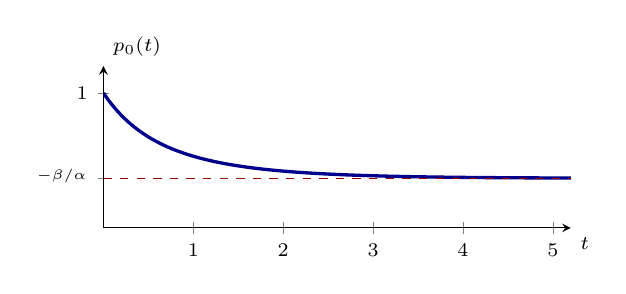
\begin{tikzpicture}
\begin{axis}[
    width=0.62\textwidth, height=0.30\textwidth,
    xlabel={$t$},
    ylabel={$p_0(t)$},
    axis lines=middle,
    xmin=0, xmax=5.2, ymin=0, ymax=1.2,
    xtick={0,1,2,3,4,5},
    ytick={0,0.36787,1},
    yticklabels={$0$,$\ee^{-\beta/\alpha}$,$1$},
    tick label style={font=\scriptsize},
    xlabel style={at={(ticklabel* cs:1)}, anchor=north west, font=\scriptsize},
    ylabel style={at={(ticklabel* cs:1)}, anchor=south west, font=\scriptsize},
]
\addplot[blue!55!black, very thick, domain=0:5.2, samples=200]
  {exp(exp(-x) - 1)};
\draw[red!60!black, dashed] (axis cs:0,0.367879) -- (axis cs:5.2,0.367879);
\end{axis}
\end{tikzpicture}
\caption{The state-zero probability \cref{m:eq:gompertzp0} at
$\beta=\alpha=1$, where it is $\ee^{\,\ee^{-t}-1}$. The curve does not decay
to zero: the dashed asymptote at $\ee^{-\beta/\alpha}$ is the probability
that the process never fires, and it is the whole difference between a
decaying rate and a constant one.}
\label{m:fig:gompertzp0}
\end{figure}

\paragraph{The mean.}
For the same process, integrating the rate gives the mean count directly:
\begin{equation}
\ex{X_t}=\int_0^t\lambda(s)\,\dd s
=\frac{\beta}{\alpha}\lrb{1-\ee^{-\alpha t}}+\gamma t,
\label{m:eq:gompertzmean}
\end{equation}
which is bounded when $\gamma=0$ and grows linearly otherwise.

\paragraph{The deterministic counterpart.}
Let $N(t)$ be a population growing at the rate \cref{m:eq:gompertzrate} and
declining at constant rate $\mu$, so that
$\ddt{N(t)}=\lrb{\lambda(t)-\mu}N(t)$. This is
\cref{m:eq:meanodeinhom} with those rates, and
\begin{equation}
N(t)=N_0\exp\lrbs{\frac{\beta}{\alpha}\lrb{1-\ee^{-\alpha t}}+(\gamma-\mu)t}.
\label{m:eq:gompertzN}
\end{equation}
Three regimes follow from the exponent. If $\mu\le\gamma$ the population
grows without bound; if $\mu\ge\gamma+\beta$ it declines from the outset;
and in between it does both.

\begin{proposition}[Rise and fall]
\label{m:prop:gompertzpeak}
If $\gamma<\mu<\gamma+\beta$ then $N(t)$ of \cref{m:eq:gompertzN} rises and
then falls, with its maximum at
\begin{equation}
t^{\ast}=\frac{1}{\alpha}\log\frac{\beta}{\mu-\gamma}.
\label{m:eq:gompertzpeak}
\end{equation}
\end{proposition}

\begin{proof}
$\dda{}{t}\log N=\lambda(t)-\mu=\beta\ee^{-\alpha t}+\gamma-\mu$, which is
strictly decreasing in $t$, is positive at $t=0$ exactly when
$\mu<\gamma+\beta$, and tends to $\gamma-\mu<0$. It therefore has a single
zero, at $\ee^{-\alpha t}=(\mu-\gamma)/\beta$.
\end{proof}

At $(\beta,\alpha,\gamma,\mu)=(2,1,0.2,0.5)$ this gives
$t^{\ast}=1.897119985$, against a numerical argmax of $1.8971$ on a
$200{,}001$-point grid.
